\documentclass[aspectratio=169]{beamer} % 16:9 aspect ratio for modern screen
% \documentclass[handout]{beamer}
% \documentclass[notes=only]{beamer}

% Theme settings
\usetheme[progressbar=foot]{metropolis} % Minimalist theme
\metroset{progressbar=frametitle} % Progress bar soll nur folien mit titel berücksichtigtigen?
\setbeamercolor{background canvas}{bg=white} % White background color

\makeatletter
    \setlength{\metropolis@progressinheadfoot@linewidth}{1.5pt}
\makeatother


\usefonttheme{professionalfonts} % Font theme

% Packages
\usepackage[T1]{fontenc}   % Font encoding
\usepackage[ngerman]{babel} % German language
\usepackage[sfdefault]{FiraSans} % For FiraSans font
\usepackage[backend=biber, style=authoryear-comp
, sorting=nyt]{biblatex} % For bibliography
\usepackage{csquotes} % Recommended for biblatex with babel/polyglossia
\usepackage{textgreek} % Greek letters in text mode (aus references von Citavi)
\usepackage{tikz}          % For drawing graphics
\usepackage{animate} % Für Animation

\usepackage{graphicx}       % For including images
\usepackage{amsmath, amssymb} % For math symbol

% \usepackage{media9} % For embedding videos

\usepackage[labelformat=empty]{caption}


% Bibliography settings
\addbibresource{references.bib} % Path to the bibliography file

% Graphics path
\graphicspath{{Images/}} % Path to images folder

% custom Citation commands
\DeclareCiteCommand{\citeauthortitle}
  {\usebibmacro{prenote}}
  {\usebibmacro{citeindex}%
   \printnames{labelname}%
   \setunit{\space\textendash\space}
   \printfield{title}}
  {\multicitedelim}
  {\usebibmacro{postnote}}

  \DeclareCiteCommand{\citeauthortitleurl}
  {\usebibmacro{prenote}}
  {\usebibmacro{citeindex}%
   \printnames{labelname}%
   \setunit{\space\textendash\space}
   \printfield{title}%
   \setunit{\addsemicolon\space}
   \printfield{url}}
  {\multicitedelim}
  {\usebibmacro{postnote}}

\DeclareCiteCommand{\parenciteauthortitle}
  {\usebibmacro{prenote}}
  {\bibopenparen\usebibmacro{citeindex}%
   \printnames{labelname}%
   \setunit{\space\textendash\space}% <- Hier wird das Trennzeichen ":" hinzugefügt
   \printfield{title}\bibcloseparen}
  {\multicitedelim}
  {\usebibmacro{postnote}}

\makeatletter
\renewcommand\footnotesize{\tiny}
\makeatother

\newcommand{\figcite}[1]{\\[-3mm]{\tiny Quelle: \cite{#1}}}
\newcommand{\figciteweb}[1]{\\[-3mm]{\tiny aus: \citeauthortitle{#1}}}
\newcommand{\figciteweburl}[1]{\\[-3mm]{\tiny aus: \citeauthortitleurl{#1}}}
  
\mode<handout>{
    \AtBeginSection[]{} % In Handout-Version keine Section-Folie erzeugen
}

% Title page settings
\title{Interactions of Charged Particles with Matter}
\subtitle{Wechselwirkungen geladener Teilchen mit Materie}
\author{Florian Marius Adamczyk}
\date{\today}
\institute{Justus-Liebig-Universität Gießen \\ Modul \textbf{Wissenschaftliches Präsentieren} bei \\ \textbf{Prof. Dr. Derck Schlettwein, PD Dr. Daniel Ebeling, Dr. Ulrike Nespital}\\
Themavergabe und Betreuer: \textbf{Dr. Roman Bergert}}
\titlegraphic{\vspace{-0.85cm}
\includegraphics[height=1.2cm]{Images/jlu_logo.jpg}}

\begin{document}

    % Black slide
    \begin{frame}<handout:0>[plain, noframenumbering]
        \begin{tikzpicture}[remember picture, overlay]
        \fill[black] (current page.south west) rectangle (current page.north east);
        \end{tikzpicture}
        \pause
        \centering
       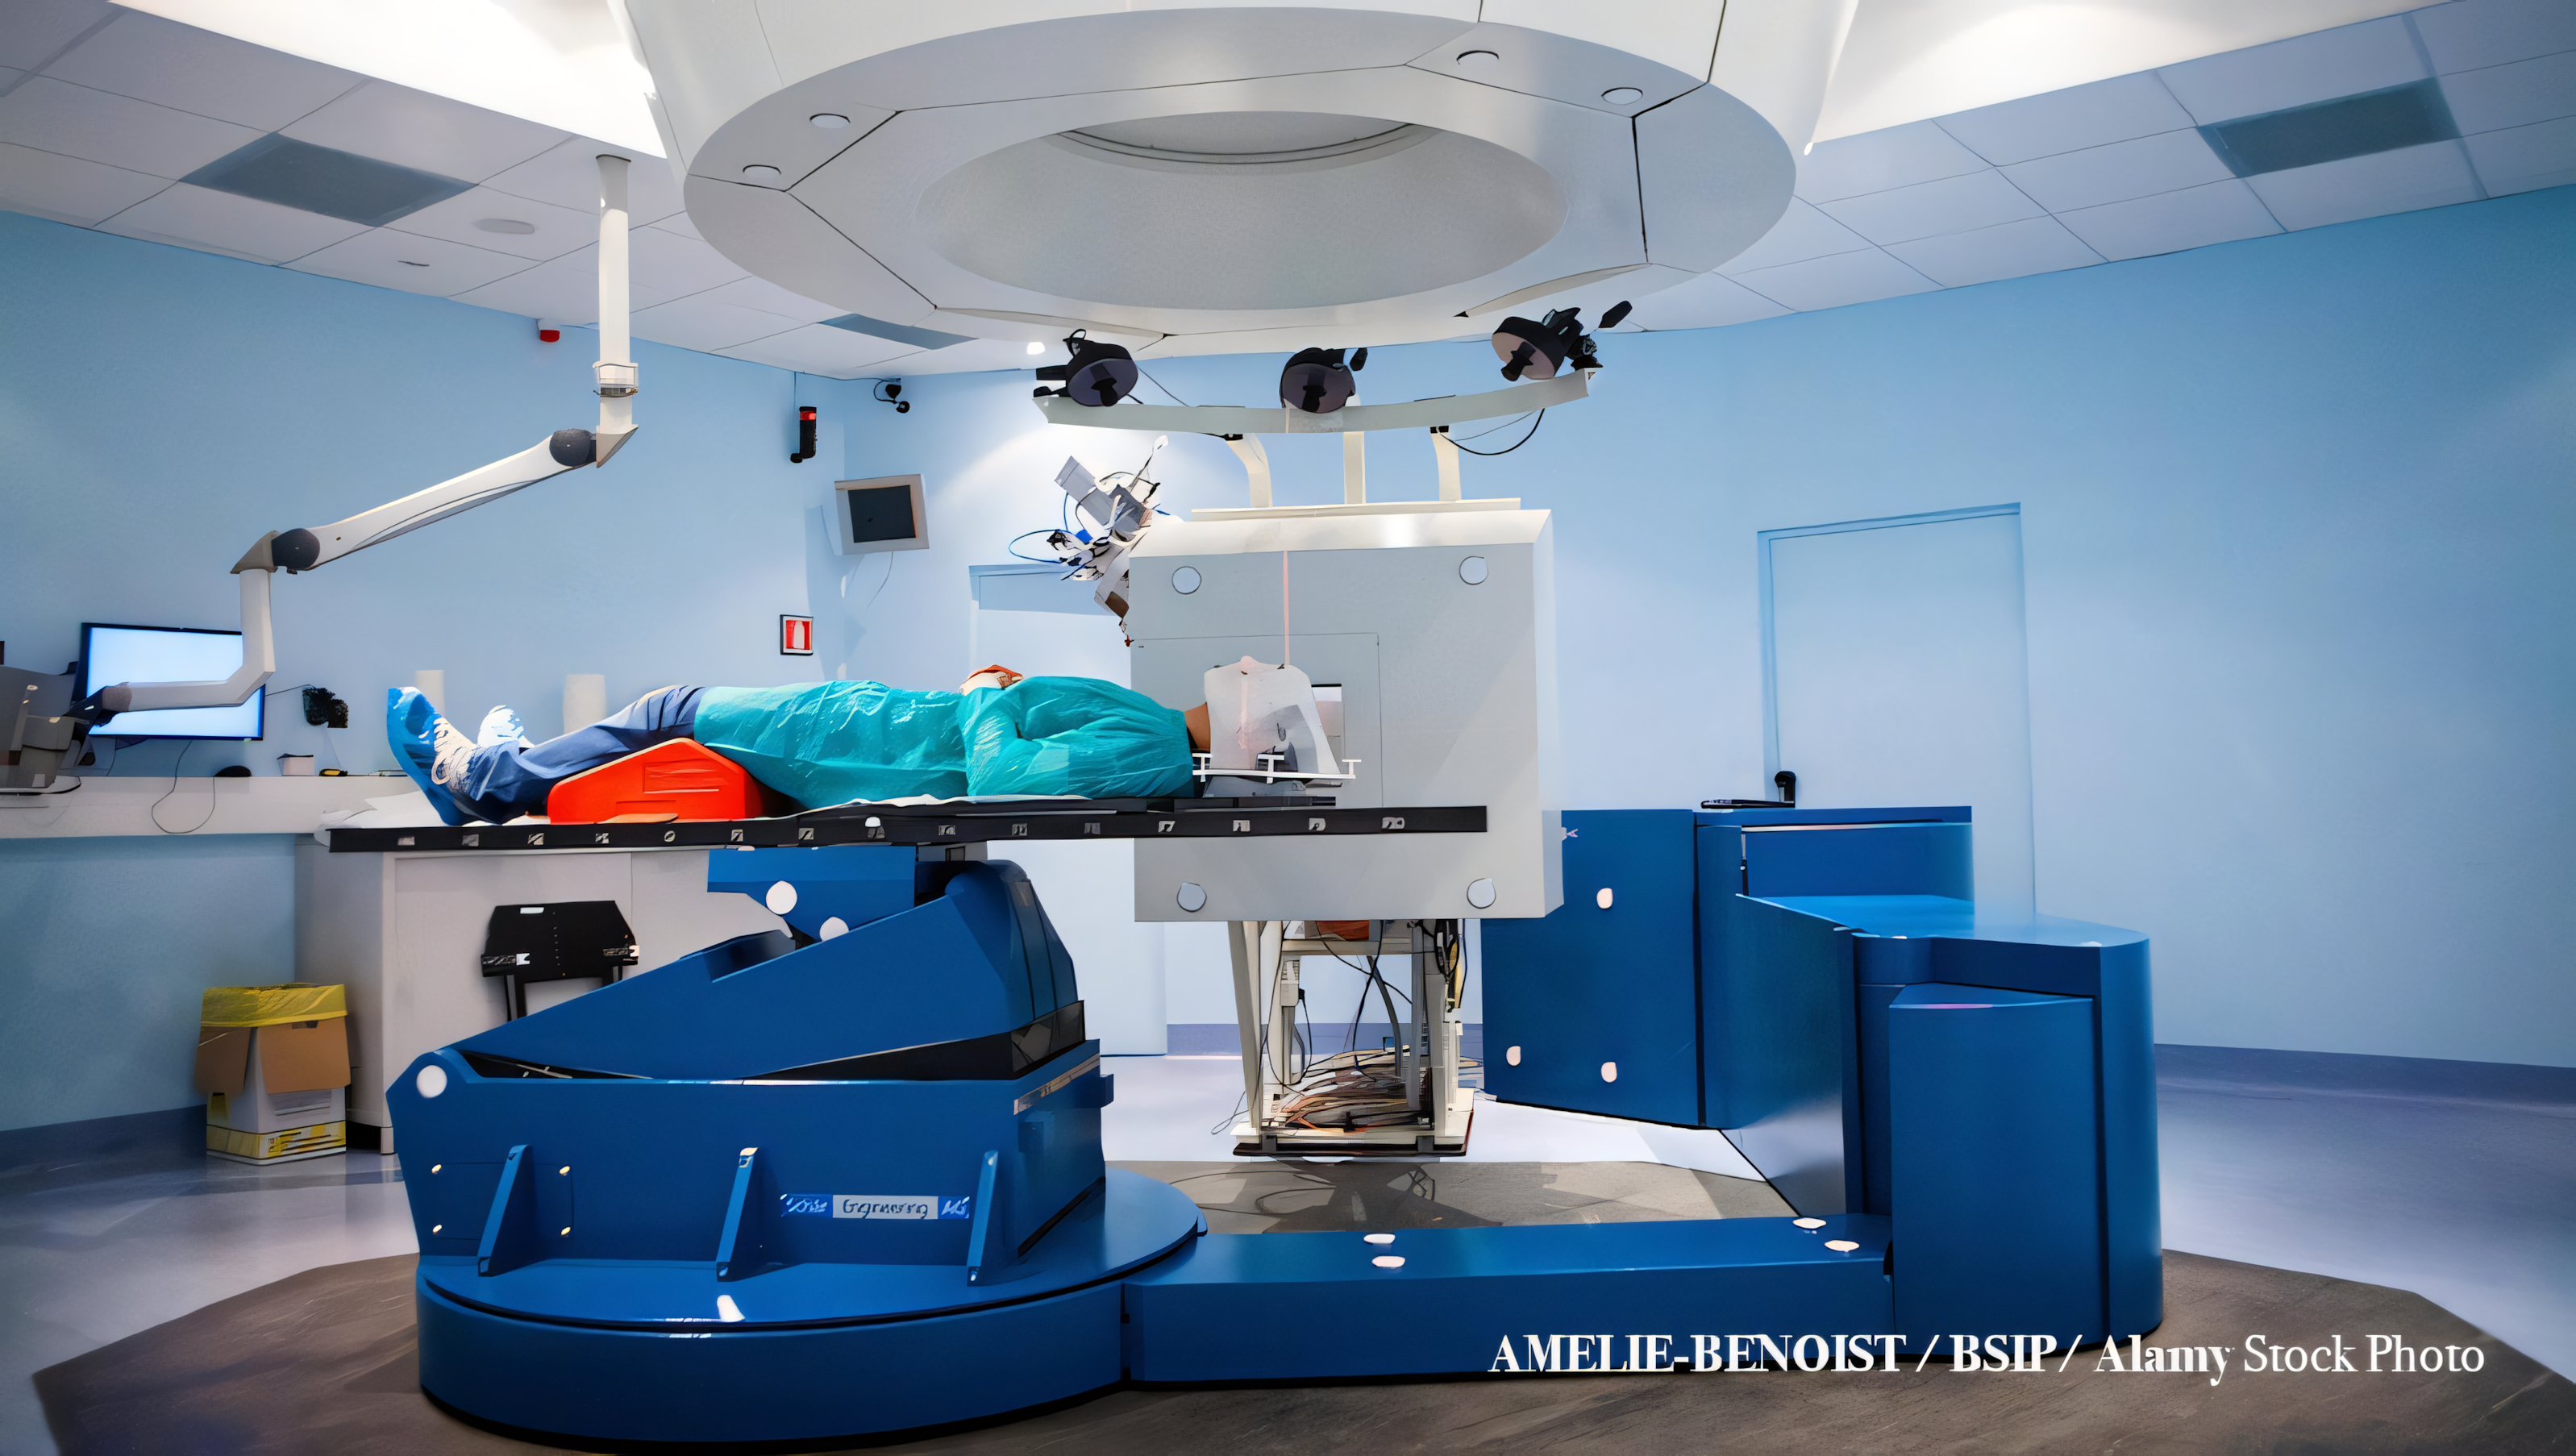
\includegraphics[width=1.0\textwidth]{Images/Titlepage.png}
    \end{frame}
   


\begin{frame}
  \titlepage
\note{\scriptsize Die pr\"azise Steuerung und Dosierung geladener Teilchen ist ein Eckpfeiler der modernen Medizinphysik. Im Kontext der Hadronentherapie--insbesondere der Protonen- oder Schwerionentherapie--entscheidet die genaue Vorhersage des Energieverlusts dar\"uber, ob der Bragg-Peak millimetergenau im Tumorgewebe platziert wird, w\"ahrend umliegendes gesundes Gewebe geschont bleibt (S.~236, Kapitel~6.4).\\[0.5ex]
Dieser kritische Bereich der Dosimetrie baut direkt auf den theoretischen Modellen auf, die erkl\"aren, wie geladene Teilchen ihre kinetische Energie schrittweise in einem absorbierenden Medium abgeben (S.~232, Abschnitt~6.2). Das Verst\"andnis des Bremsverm\"ogens ist daher nicht nur ein historisches Thema, das mit Bohr (1913) begann und mit Bethe und Fano (1930er/1960er) kulminierte, sondern es ist eine aktive Notwendigkeit f\"ur die klinische Pr\"azision (S.~230, Abschnitt~6.1).}
\end{frame}

\begin{frame}{Gliederung}
  \begin{itemize}
    \item Bremsverm\"ogen: Mechanismen und Definitionen
    \item Bethe-Formel und Dynamik des Kollisionsverlusts
    \item Gestalt der Bethe-Mass-Collision-Stopping-Power-Kurve
    \item \textcolor{gray}{(Makroskopische Konsequenzen: Bragg-Peak und Therapie)}
    \item Zusammenfassung und Ausblick
  \end{itemize}
  \note{\scriptsize 1. Einleitung: aktuelle Relevanz und Aufh\"anger (Attention Catcher).\\[0.25ex]
  2. Das Bremsverm\"ogen (Stopping Power): Mechanismen und Definitionen.\\[0.25ex]
  3. Die Bethe-Formel und die Dynamik des Kollisionsverlusts.\\[0.25ex]
  4. Die Form der Bethe Mass Collision Stopping Power Curve.\\[0.25ex]
  5. Makroskopische Konsequenzen: Der Bragg-Peak.\\[0.25ex]
  6. Zusammenfassung.}
\end{frame}

\section{Bremsverm\"ogen}

\begin{frame}{Bremsverm\"ogen: Begriffe}
  \begin{itemize}
    \item Coulomb-Wechselwirkung mit Elektronen und Kernen bestimmt Energieverlust. 
    \item Lineares Bremsverm\"ogen $(-\mathrm{d}E/\mathrm{d}x)$ beschreibt Verlust pro Wegl\"ange.
    \item Massenbremsverm\"ogen $S = -\frac{1}{\rho}\frac{\mathrm{d}E}{\mathrm{d}x}$ setzt auf Absorberdichte ab.
    \item Gesamtterm: $S_{\text{tot}} = S_{\text{col}} + S_{\text{rad}}$.
  \end{itemize}
  \note{\scriptsize Ein geladenes Teilchen, das in Materie eindringt, ist von seinem Coulomb-Feld umgeben, welches sowohl mit den Orbitalelektronen als auch mit den Atomkernen des Absorbers wechselwirkt. Die resultierenden Energie\"ubertr\"age bestimmen, wie schnell das Teilchen seine kinetische Energie verliert--genau diese Verlustleistung fasst das Bremsverm\"ogen (S.~229).\\[0.5ex]
  Das lineare Bremsverm\"ogen beschreibt den Energieverlust pro Einheitsweg $(-\mathrm{d}E/\mathrm{d}x)$ in \si{MeV\per\centi\metre}. Teilt man diesen Ausdruck durch die Dichte $\rho$ des Absorbers, erh\"alt man das Massenbremsverm\"ogen $S = -\frac{1}{\rho}\frac{\mathrm{d}E}{\mathrm{d}x}$ mit der Einheit \si{MeV\centi\metre\squared\per\gram} (S.~232~ff.).\\[0.5ex]
  Das Gesamt-Massenbremsverm\"ogen setzt sich additiv aus Kollisions- und Strahlungsanteil zusammen: $S_{\text{tot}} = S_{\text{col}} + S_{\text{rad}}$ (S.~233).}
\end{frame}

\begin{frame}{Strahlungsverlust und Sto\ss{}parameter}
  \begin{columns}[T,totalwidth=\textwidth]
    \begin{column}{0.58\textwidth}
      \begin{itemize}
        \item Strahlungsverlust entsteht durch Bremsstrahlung bei Kernn\"aherung.
        \item Beitrag w\"achst mit kinetischer Energie und skaliert wie $Z^2$ des Absorbers.
        \item Proportional zu $1/m^2$ des Projektils; f\"ur schwere Ionen meist vernachl\"assigbar.
        \item Kritische Energie $E_{K,\text{crit}}$ markiert Gleichgewicht von $S_{\text{rad}}$ und $S_{\text{col}}$.
      \end{itemize}
    \end{column}
    \begin{column}{0.42\textwidth}
      \begin{figure}
        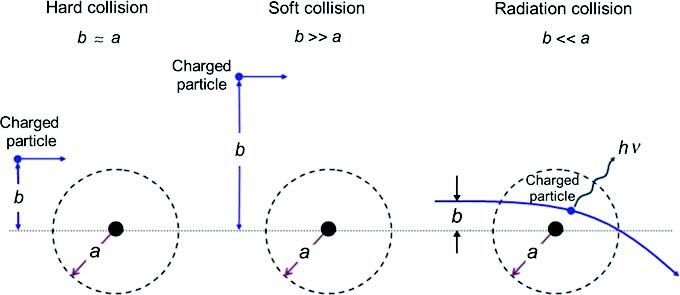
\includegraphics[width=\textwidth]{Images/CollisionTypes.jpeg}
        \caption{Kollisionsarten nach Sto\ss{}parameter}
      \end{figure}
    \end{column}
  \end{columns}
  \note{\scriptsize Der Strahlungsverlust beschreibt die Energieabgabe durch Bremsstrahlung infolge der Wechselwirkung mit den Atomkernen des Absorbers (S.~233).\\[0.5ex]
  Bei sehr kleinem Sto\ss{}parameter gegen\"uber dem Atomradius ($b \ll a$) wird das Projektil vom Atomkern stark abgelenkt und emittiert Bremsstrahlung. Die mittlere Verlustleistung w\"achst mit der kinetischen Energie, skaliert nahezu quadratisch mit der Kernladungszahl des Absorbers ($\propto Z^2$) und f\"allt mit dem Quadrat der Teilchenmasse ($\propto 1/m^2$). F\"ur Elektronen/Positronen kann der Strahlungsanteil daher den Kollisionsanteil \"ubersteigen; f\"ur Protonen und schwerere Ionen bleibt er vernachl\"assigbar. Der \"Ubergangspunkt, an dem Strahlung und Kollision gleich wichtig werden, ist die kritische Energie $E_{K,\text{crit}}$.}
\end{frame}

\begin{frame}{Kollisionsverlust: Komponenten}
  \begin{columns}[T,totalwidth=\textwidth]
    \begin{column}{0.58\textwidth}
      \begin{itemize}
    \item Kollisionsverluste dominieren f\"ur schwere Projektile (Electronic Stopping).
    \item Zerlegung in weiche und harte Beitr\"age: $S_{\text{col}} = S_{\text{soft}}^{\text{col}} + S_{\text{hard}}^{\text{col}}$.
    \item Weiche Kollisionen ($b \gg a$) liefern h\"aufige, kleine Energie\"ubertr\"age.
    \item Harte Kollisionen ($b \approx a$) erzeugen $\delta$-Elektronen und gro\ss{}e Energieverluste.
  \end{itemize}
    \end{column}
    \begin{column}{0.42\textwidth}
      \begin{figure}
        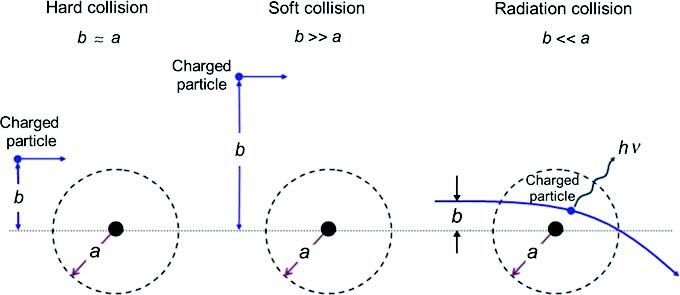
\includegraphics[width=\textwidth]{Images/CollisionTypes.jpeg}
        \caption{Kollisionsarten nach Sto\ss{}parameter}
      \end{figure}
    \end{column}
  \end{columns}
  \note{\scriptsize Der Kollisionsverlust beschreibt die mittlere Energieabgabe an Orbitalelektronen und f\"uhrt zu Anregung oder Ionisation (Electronic Stopping Power). F\"ur schwere Projektile ist dies der dominante Term, da der Strahlungsanteil unterdr\"uckt ist. In der Praxis wird der Kollisionsverlust in weiche und harte Beitr\"age zerlegt: $S_{\text{col}} = S_{\text{soft}}^{\text{col}} + S_{\text{hard}}^{\text{col}}$.\\[0.5ex]
  Die mikroskopischen Wechselwirkungen werden klassisch \"uber den Sto\ss{}parameter $b$ relativ zum Atomradius $a$ charakterisiert (S.~230).\\[0.5ex]
  1. Weiche (distant) Kollisionen ($b \gg a$): Das Teilchen sp\"urt das gesamte Atom, der Energie\"ubertrag pro Ereignis ist klein, die H\"aufigkeit jedoch gro\ss{}. Diese Prozesse f\"uhren zu Polarisation, Anregung und Ionisation und tragen rund die H\"alfte zu $S_{\text{col}}$ bei.\\[0.25ex]
   2. Harte (close) Kollisionen ($b \approx a$): Direkte Coulomb-Wechselwirkung an einzelnen Elektronen verursacht gro\ss{}e Energie\"ubertr\"age. Die ausgel\"osten $\delta$-Elektronen sind selbst ionisierend und liefern den restlichen Beitrag zu $S_{\text{col}}$.}
\end{frame}

\section{Bethe-Formel}

\begin{frame}{Bethe-Gleichung}
  \begin{equation*}
    S_{\text{col}} = C_0 \frac{z^2}{A\beta^2} Z \left\{ \ln \frac{2 m_e c^2}{I} + \ln \frac{\beta^2}{1 - \beta^2} - \beta^2 \right\}
  \end{equation*}
  \begin{itemize}
    \item \textbf{Teilchenparameter}: $z^2$ und $1/\beta^2$ treiben Anstieg bei langsamen Projektilen.
        \item \textbf{Materialeigenschaften}: Elektronendichte $Z/A$ und gemittelte Ionisationsenergie $I$.
        \item \textbf{Relativistische Terme}: $\ln \frac{\beta^2}{1-\beta^2} - \beta^2$ f\"uhren zu Hochenergieanstieg.
  \end{itemize}
  \note{\scriptsize Bethe unterteilte $S_{\text{col}}$ in $S_{\text{soft}}$ und $S_{\text{hard}}$. Bei der Zusammenfassung der Terme (Gleichung~6.40 und~6.41) f\"allt die willk\"urlich gew\"ahlte Energieabgrenzung $\eta$ zwischen weichen und harten Kollisionen heraus.\\[0.5ex]
  Das Ergebnis f\"ur schwere geladene Teilchen (Bethe Mass Collision Stopping Power Equation) lautet ohne Korrekturen: $S_{\text{col}} = C_0 \frac{z^2}{A\beta^2} Z \{ \ln \frac{2 m_e c^2}{I} + \ln \frac{\beta^2}{1-\beta^2} - \beta^2 \}$ (S.~246).}
\end{frame}

\begin{frame}{Terminterpretation und Korrekturen}
  \begin{columns}[T,totalwidth=\textwidth]
    \begin{column}{0.6\textwidth}
      \begin{itemize}
        
        \item \textbf{Korrekturen}: Schalenkorrektur $C/Z$ (niedrige Energien), Dichteeffekt $\delta$ (hohe Energien).
      \end{itemize}
    \end{column}
    \begin{column}{0.4\textwidth}
      \begin{figure}
        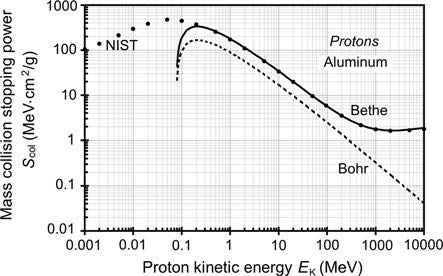
\includegraphics[width=\textwidth]{Images/BetheKorr.jpeg}
        \caption{Korrekturterme der Bethe-Formel}
      \end{figure}
    \end{column}
  \end{columns}
  \note{\scriptsize \begin{enumerate}
    \item Teilchenladung und Geschwindigkeitsterm: $C_0 \frac{z^2}{A\beta^2} Z$ zeigt, dass die Bremskraft proportional zum Quadrat der Ladung des Projektils ist, w\"ahrend sie im nicht-relativistischen und intermedi\"aren Bereich umgekehrt proportional zum Quadrat der Teilchengeschwindigkeit ($\beta = v/c$) bleibt.\\
    \item Absorber-Eigenschaften: Die Elektronendichte $N_e = Z N_A / A$ des Absorbers bestimmt die Anzahl der Wechselwirkungspartner. Da $Z/A$ f\"ur die meisten Elemente nahe~0.5 liegt, variiert $S_{\text{col}}$ nur wenig zwischen verschiedenen Materialien. Das mittlere Ionisationspotential $I$ ist die minimale Energie f\"ur eine Wechselwirkung und wird empirisch bestimmt.\\
    \item Relativistische Terme: $\ln \frac{\beta^2}{1-\beta^2} - \beta^2$ gewinnen an Bedeutung, wenn $\beta$ gegen~1 geht und erzeugen den langsamen Wiederanstieg der Bremskraft bei sehr hohen Energien.
  \end{enumerate}
  Um die \"Ubereinstimmung mit Messdaten zu verbessern, insbesondere bei niedrigen Energien und in kondensierten Medien, werden der Bethe-Formel Korrekturen hinzugef\"ugt: die Shell Correction $C/Z$ bei niedriger Energie (wenn die Teilchengeschwindigkeit vergleichbar mit der Elektronengeschwindigkeit ist) und die Density-Effect Correction $\delta$ bei hohen Energien aufgrund der Polarisation des Mediums.}
\end{frame}

\section{Bethe-Kurve}

\begin{frame}{Bethe-Kurve: Charakteristische Regionen}
  \begin{columns}[T,totalwidth=\textwidth]
    \begin{column}{0.55\textwidth}
      \begin{itemize}
        \item Region 1: Anstieg des $S_{\text{col}}$ bei niedrigen Energien bis zum Maximum.
        \item Region 2: Minimum Ionizing Particle (MIP) bei intermedi\"aren Energien.
        \item Region 3: Relativistischer Wiederanstieg mit Dichteeffekt in festen Medien.
      \end{itemize}
    \end{column}
    \begin{column}{0.45\textwidth}
      \begin{figure}
        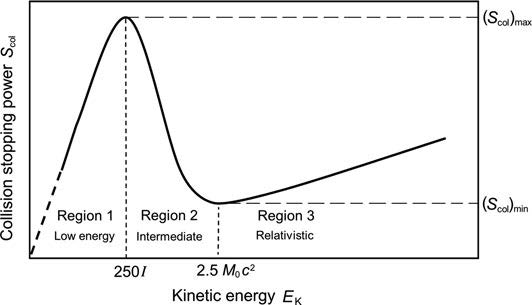
\includegraphics[width=\textwidth]{Images/BetheCurve.jpeg}
        \caption{Bethe-Mass-Collision-Stopping-Power-Kurve}
      \end{figure}
    \end{column}
  \end{columns}
  \note{\scriptsize Die Auftragung des Kollisionsbremsverm\"ogens $S_{\text{col}}$ als Funktion der kinetischen Energie $E_K$ f\"ur schwere geladene Teilchen zeigt drei charakteristische Regionen (S.~249).\\[0.5ex]
  Region~1: Niedrige Energie. $S_{\text{col}}$ steigt mit $E_K$ an und erreicht ein Maximum. Die klassische Bethe-Theorie bricht hier ab; Schalenkorrekturen werden notwendig. Das Maximum tritt experimentell etwa bei $E_K \approx 250 I$ auf.\\[0.25ex]
  Region~2: Intermedi\"are Energie (MIP-Region). Jenseits des Maximums f\"allt $S_{\text{col}}$ schnell ab, proportional zu $1/\beta^2$ und erreicht ein breites Minimum, nahezu materialunabh\"angig bei $E_K \approx 2.5 M_0 c^2$.\\[0.25ex]
  Region~3: Relativistische Energie. Jenseits des Minimums steigt $S_{\text{col}}$ langsam wieder an. Der Dichteeffekt $\delta$ saturiert den Anstieg in kondensierten Medien.}
\end{frame}

\begin{frame}{Kernaussagen}
  \begin{columns}[T,totalwidth=\textwidth]
    \begin{column}{0.55\textwidth}
      \begin{itemize}
        \item Energieverlust geladener Teilchen entsteht durch $S_{\text{col}}$ und $S_{\text{rad}}$.
        \item Bethe-Kurve zeigt Maximum, MIP-Minimum und relativistischen Anstieg.
        \item Gezielte Formung des Bragg-Peaks erm\"oglicht pr\"azise Hadronentherapie.
      \end{itemize}
    \end{column}
    \begin{column}{0.45\textwidth}
      \begin{figure}
        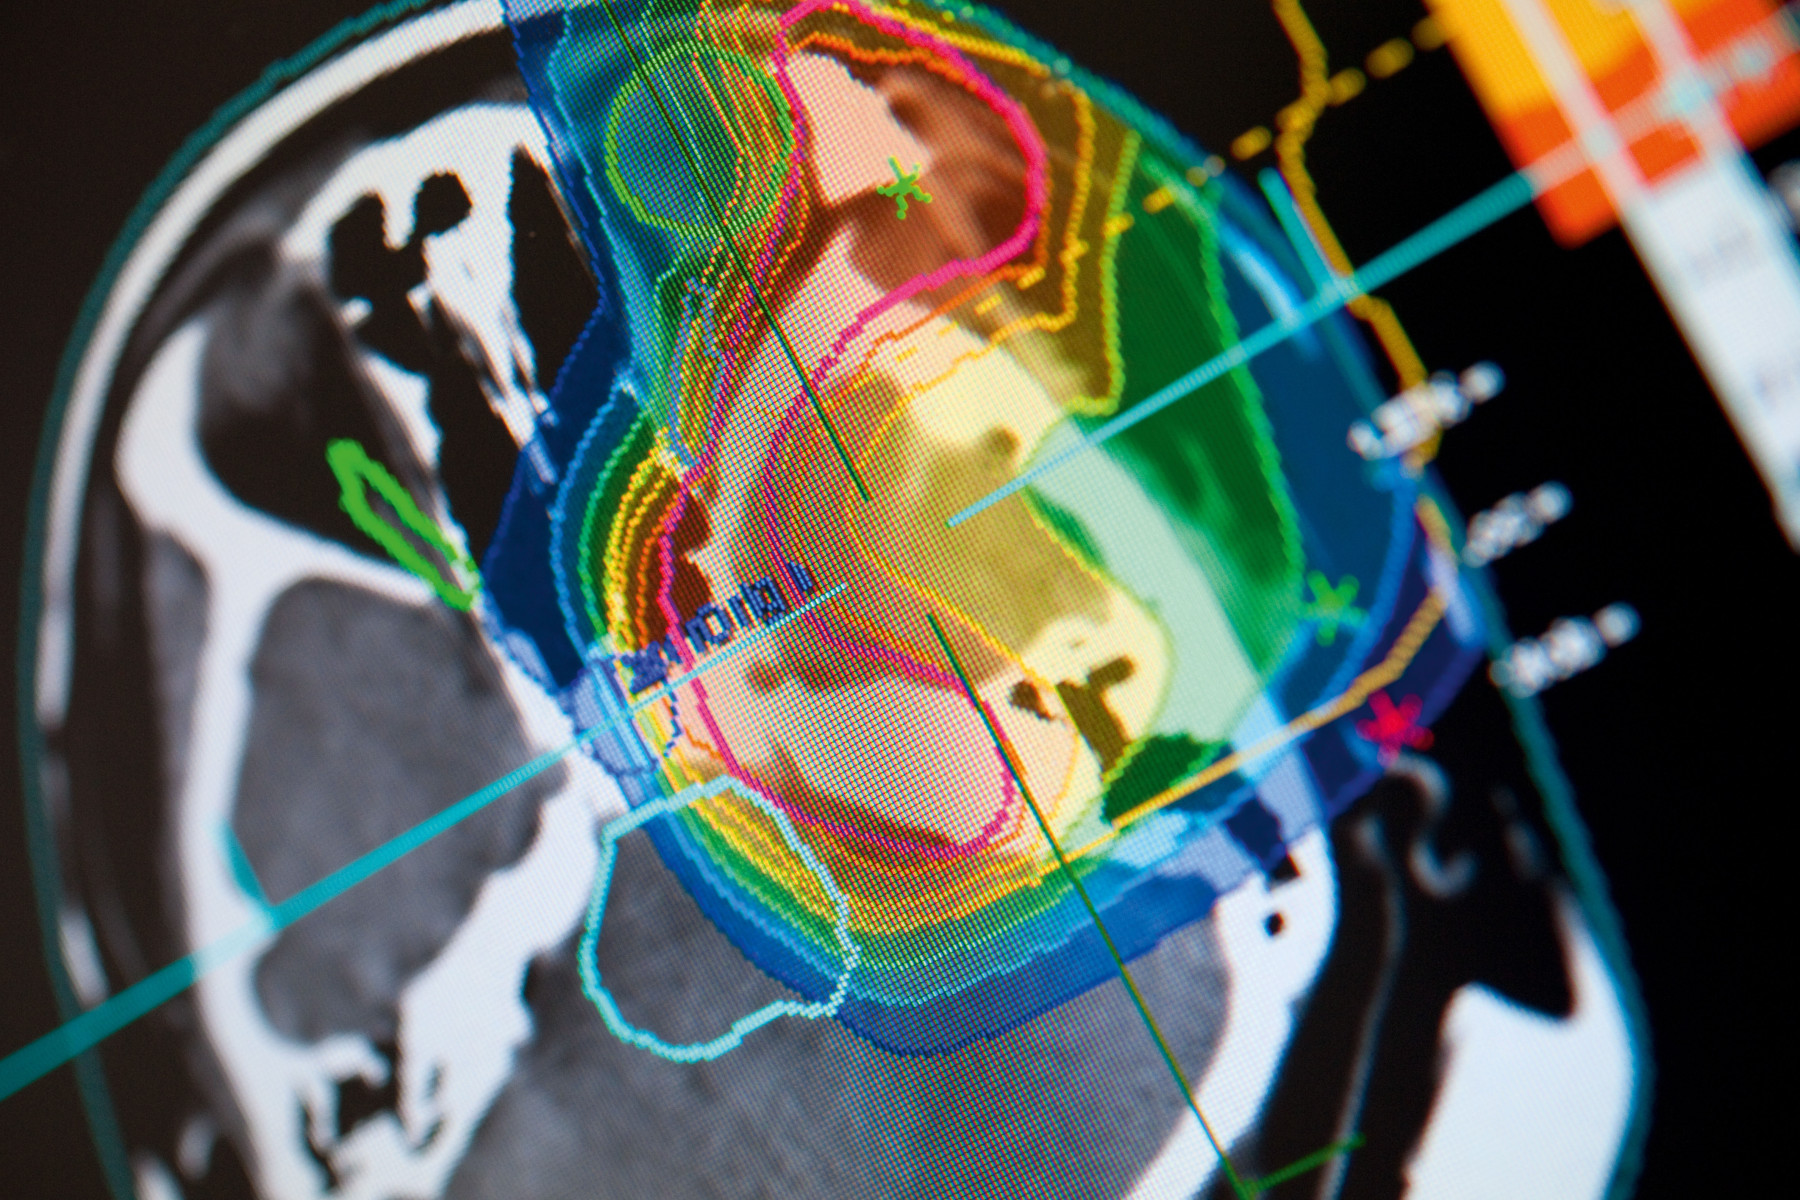
\includegraphics[width=\textwidth]{Images/1920_hirntumorbestrahlung.jpg}
        \caption{Klinische Anwendung des Bragg-Peaks}
      \end{figure}
    \end{column}
  \end{columns}
  \note{\scriptsize Die Wechselwirkungen geladener Teilchen mit Materie sind durch zwei Hauptmechanismen definiert: den Kollisionsverlust $S_{\text{col}}$ mit Orbitalelektronen und den Strahlungsverlust $S_{\text{rad}}$ mit Atomkernen. Das Bremsverm\"ogen $S$ ist die quantitative Beschreibung dieser Energieverlustrate.\\[0.5ex]
  F\"ur schwere geladene Teilchen wird $S_{\text{col}}$ prim\"ar durch die Bethe-Formel beschrieben, welche die Abh\"angigkeit von der Teilchengeschwindigkeit \"uber den $1/\beta^2$-Term und die Materialeigenschaften \"uber die mittlere Ionisationsenergie $I$ darstellt. Die Bethe-Kurve zeigt einen $1/\beta^2$-Abfall bei mittleren Energien, gefolgt von einem Minimum (MIP-Region bei $E_K \approx 2.5 M_0 c^2$) und einem relativistischen Anstieg.\\[0.5ex]
  Die pr\"azise Kenntnis dieser theoretischen Grundlagen erm\"oglicht es, makroskopische Ph\"anomene wie den Bragg-Peak zu modellieren. Die F\"ahigkeit, den Bragg-Peak zu formen und pr\"azise im Zielvolumen zu platzieren, definiert die moderne Hadronentherapie und bildet die Grundlage f\"ur die Dosimetrie in der Medizinphysik. Die Forschung in diesem Bereich bleibt essenziell, um die klinische Pr\"azision fortlaufend zu optimieren.}
\end{frame}

\begin{frame}<handout:0>[plain, noframenumbering]
        \begin{tikzpicture}[remember picture, overlay]
          \fill[black] (current page.south west) rectangle (current page.north east);
        \end{tikzpicture}
\end{frame}

\section{Bragg-Peak}

\begin{frame}[noframenumbering]{Bragg-Peak: Mechanismus}
  \begin{columns}[T,totalwidth=\textwidth]
    \begin{column}{0.55\textwidth}
      \begin{itemize}
        \item Schwerionen verlieren Energie nahezu ausschlie\ss{}lich durch Kollisionen.
        \item $S_{\text{col}} \propto 1/\beta^2$ f\"uhrt zu starker Dosisabgabe kurz vor Stillstand.
        \item Energiedeposition bildet ausgepr\"agten Bragg-Peak am Ende der Reichweite.
      \end{itemize}
    \end{column}
    \begin{column}{0.45\textwidth}
      \begin{figure}
        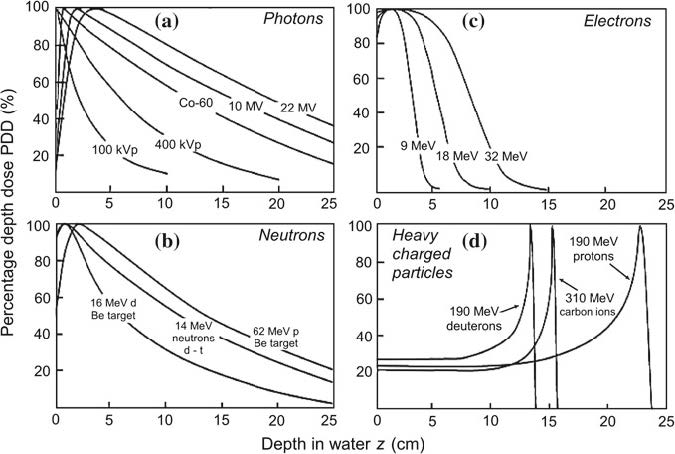
\includegraphics[width=\textwidth]{Images/BraggPeak.jpeg}
        \caption{Energieabgabe nach Tiefe f\"ur verschiedene Teilchen}
      \end{figure}
    \end{column}
  \end{columns}
    \note{\scriptsize Nachdem wir die mikroskopische und relativistische Theorie des Energieverlusts analysiert haben, betrachten wir die makroskopische Manifestation dieses Energieabgabezustands bei schweren geladenen Teilchen wie Protonen oder Alpha-Teilchen. Der Energieverlust erfolgt nahezu ausschlie\ss{}lich durch Kollisionen; der Strahlungsverlust ist vernachl\"assigbar, sodass die Teilchen nahezu geradlinig bleiben.\\[0.5ex]
    Der Bragg-Peak beschreibt den ausgepr\"agten Anstieg der Energiedepositionsrate am Ende des Teilchenpfades. Dieser Peak ist die direkte Folge der Proportionalit\"at der Kollisionsbremskraft zur reziproken Teilchengeschwindigkeit im intermedi\"aren Bereich ($S_{\text{col}} \propto 1/\beta^2$). W\"ahrend das Teilchen Materie durchquert und Energie verliert, verlangsamt es sich und $S_{\text{col}}$ steigt dramatisch, sodass kurz vor dem Stillstand ein Maximum der Dosisabgabe erreicht wird (S.~24).}
\end{frame}

\begin{frame}[noframenumbering]{Klinische Relevanz der Hadronentherapie}
  \begin{columns}[T,totalwidth=\textwidth]
    \begin{column}{0.55\textwidth}
      \begin{itemize}
        \item Bragg-Peak erlaubt millimetergenaue Dosisdeposition im Tumorvolumen.
        \item Eintrittsdosis bleibt gering, distal kaum Restdosis im gesunden Gewebe.
        \item Vorteil gegen\"uber Photonen: steiler Dosisabfall hinter dem Zielvolumen.
      \end{itemize}
    \end{column}
    \begin{column}{0.45\textwidth}
      \begin{figure}
        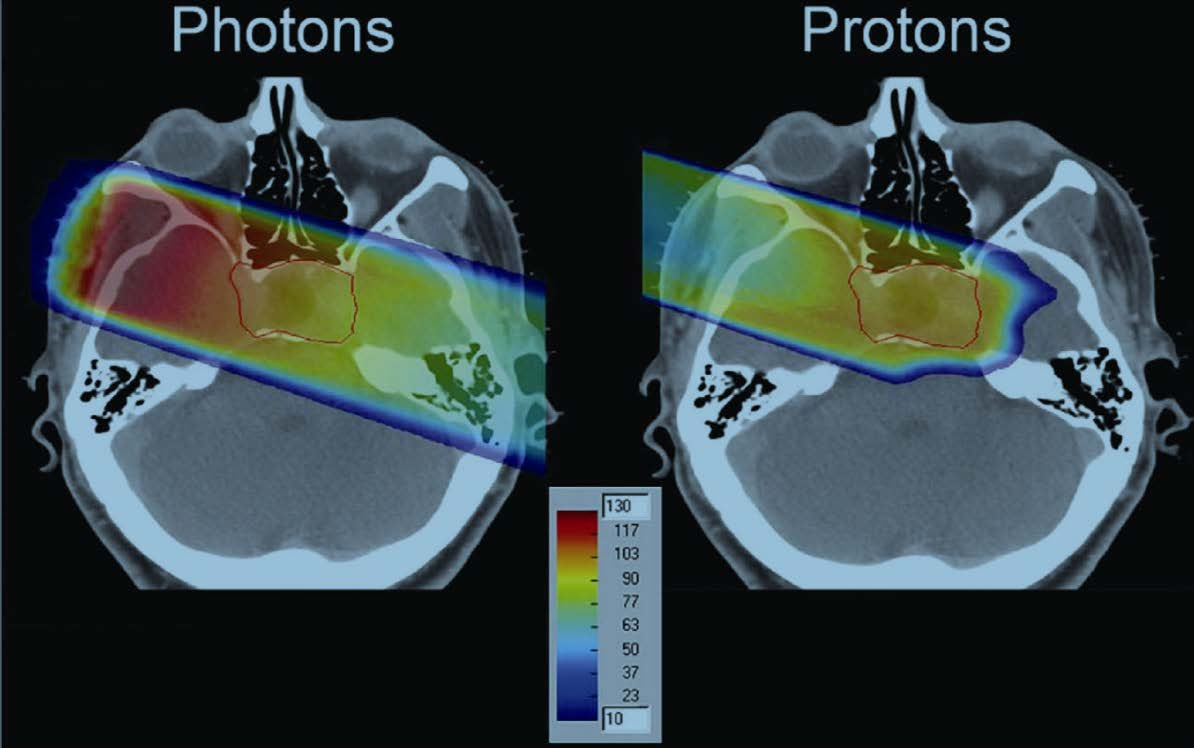
\includegraphics[width=\textwidth]{Images/DSD_88.jpg}
        \caption{Dosisprofil in der Hadronentherapie}
      \end{figure}
    \end{column}
  \end{columns}
  \note{\scriptsize Die einzigartige Eigenschaft des Bragg-Peaks--n\"amlich die scharfe Abgrenzung der Dosisdeponierung in einer spezifischen Tiefe--ist der zentrale Vorteil der Hadronentherapie gegen\"uber der konventionellen Photonentherapie. Im Gegensatz zu energiereichen Photonenstrahlen, deren Dosis exponentiell oder asymptotisch abf\"allt, erlaubt die Bragg-Peak-Kurve eine millimetergenaue Dosierung des Tumors, w\"ahrend das davor liegende Gewebe nur eine geringere Eintrittsdosis erh\"alt und das dahinterliegende Gewebe nahezu vollst\"andig geschont wird.}
\end{frame}

\begin{frame}[noframenumbering]{Spread-Out Bragg Peak (SOBP)}
  \begin{columns}[T,totalwidth=\textwidth]
    \begin{column}{0.6\textwidth}
      \begin{itemize}
        \item Monoenergetischer Peak ist schmal und f\"ur gro\ss{}e Tumoren zu eng.
        \item Energie-Modulation (spinning wedges, Filter) erzeugt SOBP-Plateau.
        \item Anpassung der Dosis an dreidimensionale Tumorgeometrie.
      \end{itemize}
    \end{column}
    \begin{column}{0.4\textwidth}
      \begin{figure}
        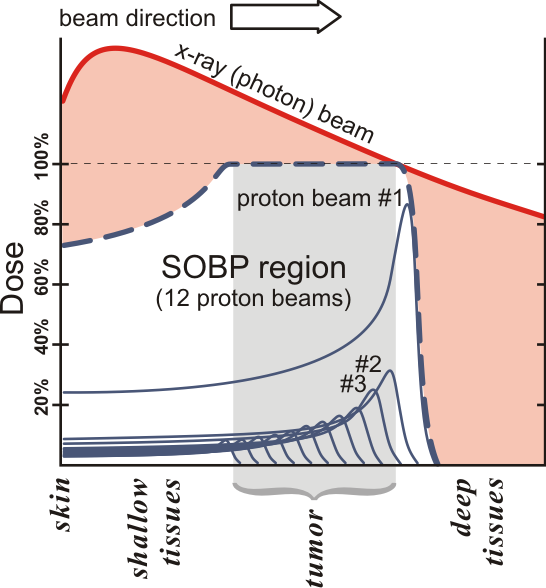
\includegraphics[width=\textwidth]{Images/SOBP.png}
        \caption{Geformter Spread-Out Bragg Peak}
      \end{figure}
    \end{column}
  \end{columns}
  \note{\scriptsize Der Bragg-Peak eines monoenergetischen Strahls ist sehr schmal. Um gr\"o\ss{}ere Tumoren klinisch behandeln zu k\"onnen, muss dieser Peak verbreitert werden. Dies wird durch die Erzeugung eines Spread-Out Bragg Peak (SOBP) erreicht, indem man einen Strahl mit einer verteilten Energie verwendet, etwa durch variable Dicke von Abschw\"achern (spinning wedges). Die Modifikation des monoenergetischen Strahls resultiert in einem Plateau, das der spezifischen 3D-Form des Tumors angepasst werden kann.}
\end{frame}

\begin{frame}[noframenumbering]{Kernaussagen}
  \begin{columns}[T,totalwidth=\textwidth]
    \begin{column}{0.55\textwidth}
      \begin{itemize}
        \item Energieverlust geladener Teilchen entsteht durch $S_{\text{col}}$ und $S_{\text{rad}}$.
        \item Bethe-Kurve zeigt Maximum, MIP-Minimum und relativistischen Anstieg.
        \item Gezielte Formung des Bragg-Peaks erm\"oglicht pr\"azise Hadronentherapie.
      \end{itemize}
    \end{column}
    \begin{column}{0.45\textwidth}
      \begin{figure}
        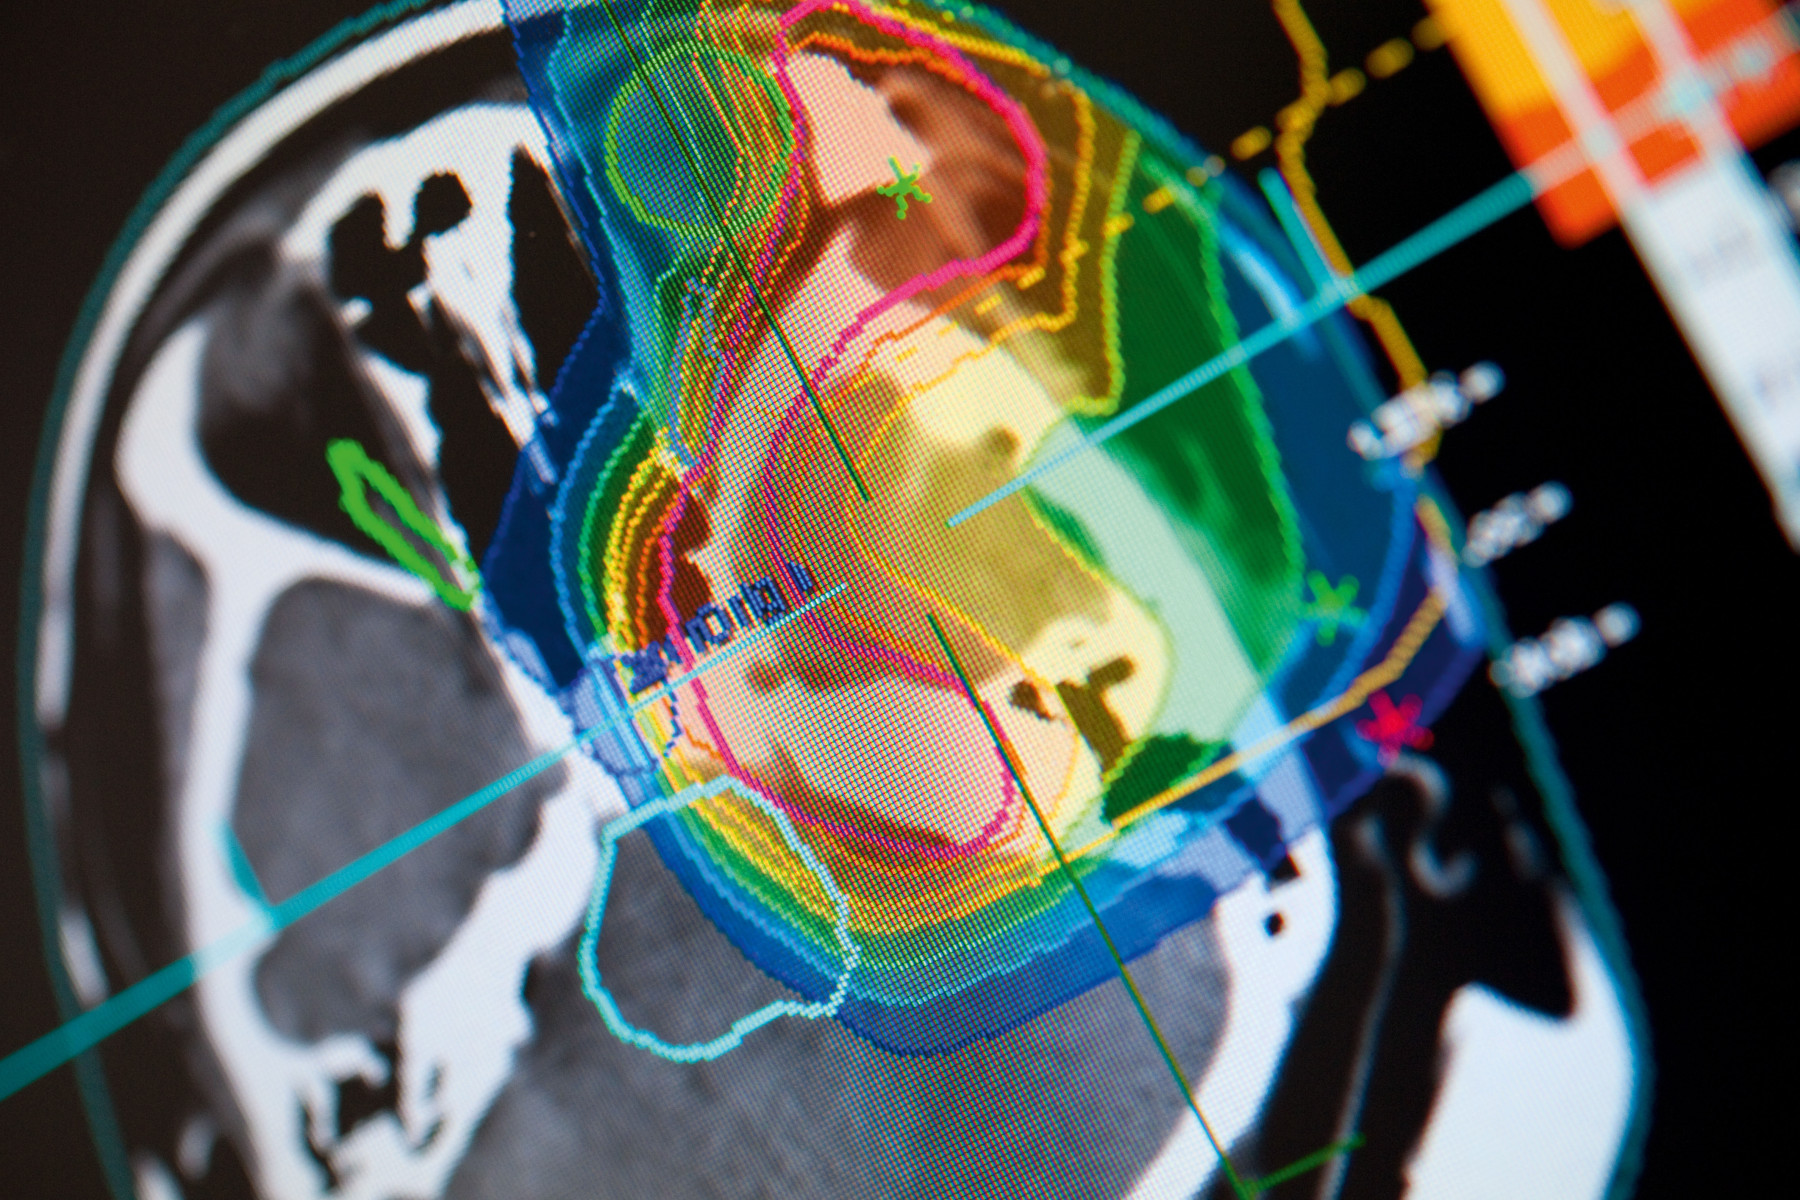
\includegraphics[width=\textwidth]{Images/1920_hirntumorbestrahlung.jpg}
        \caption{Klinische Anwendung des Bragg-Peaks}
      \end{figure}
    \end{column}
  \end{columns}
  \note{\scriptsize Die Wechselwirkungen geladener Teilchen mit Materie sind durch zwei Hauptmechanismen definiert: den Kollisionsverlust $S_{\text{col}}$ mit Orbitalelektronen und den Strahlungsverlust $S_{\text{rad}}$ mit Atomkernen. Das Bremsverm\"ogen $S$ ist die quantitative Beschreibung dieser Energieverlustrate.\\[0.5ex]
  F\"ur schwere geladene Teilchen wird $S_{\text{col}}$ prim\"ar durch die Bethe-Formel beschrieben, welche die Abh\"angigkeit von der Teilchengeschwindigkeit \"uber den $1/\beta^2$-Term und die Materialeigenschaften \"uber die mittlere Ionisationsenergie $I$ darstellt. Die Bethe-Kurve zeigt einen $1/\beta^2$-Abfall bei mittleren Energien, gefolgt von einem Minimum (MIP-Region bei $E_K \approx 2.5 M_0 c^2$) und einem relativistischen Anstieg.\\[0.5ex]
  Die pr\"azise Kenntnis dieser theoretischen Grundlagen erm\"oglicht es, makroskopische Ph\"anomene wie den Bragg-Peak zu modellieren. Die F\"ahigkeit, den Bragg-Peak zu formen und pr\"azise im Zielvolumen zu platzieren, definiert die moderne Hadronentherapie und bildet die Grundlage f\"ur die Dosimetrie in der Medizinphysik. Die Forschung in diesem Bereich bleibt essenziell, um die klinische Pr\"azision fortlaufend zu optimieren.}
\end{frame}

\begin{frame}[noframenumbering]{Interactions of Charged Particles with Matter}
  \begin{figure}
        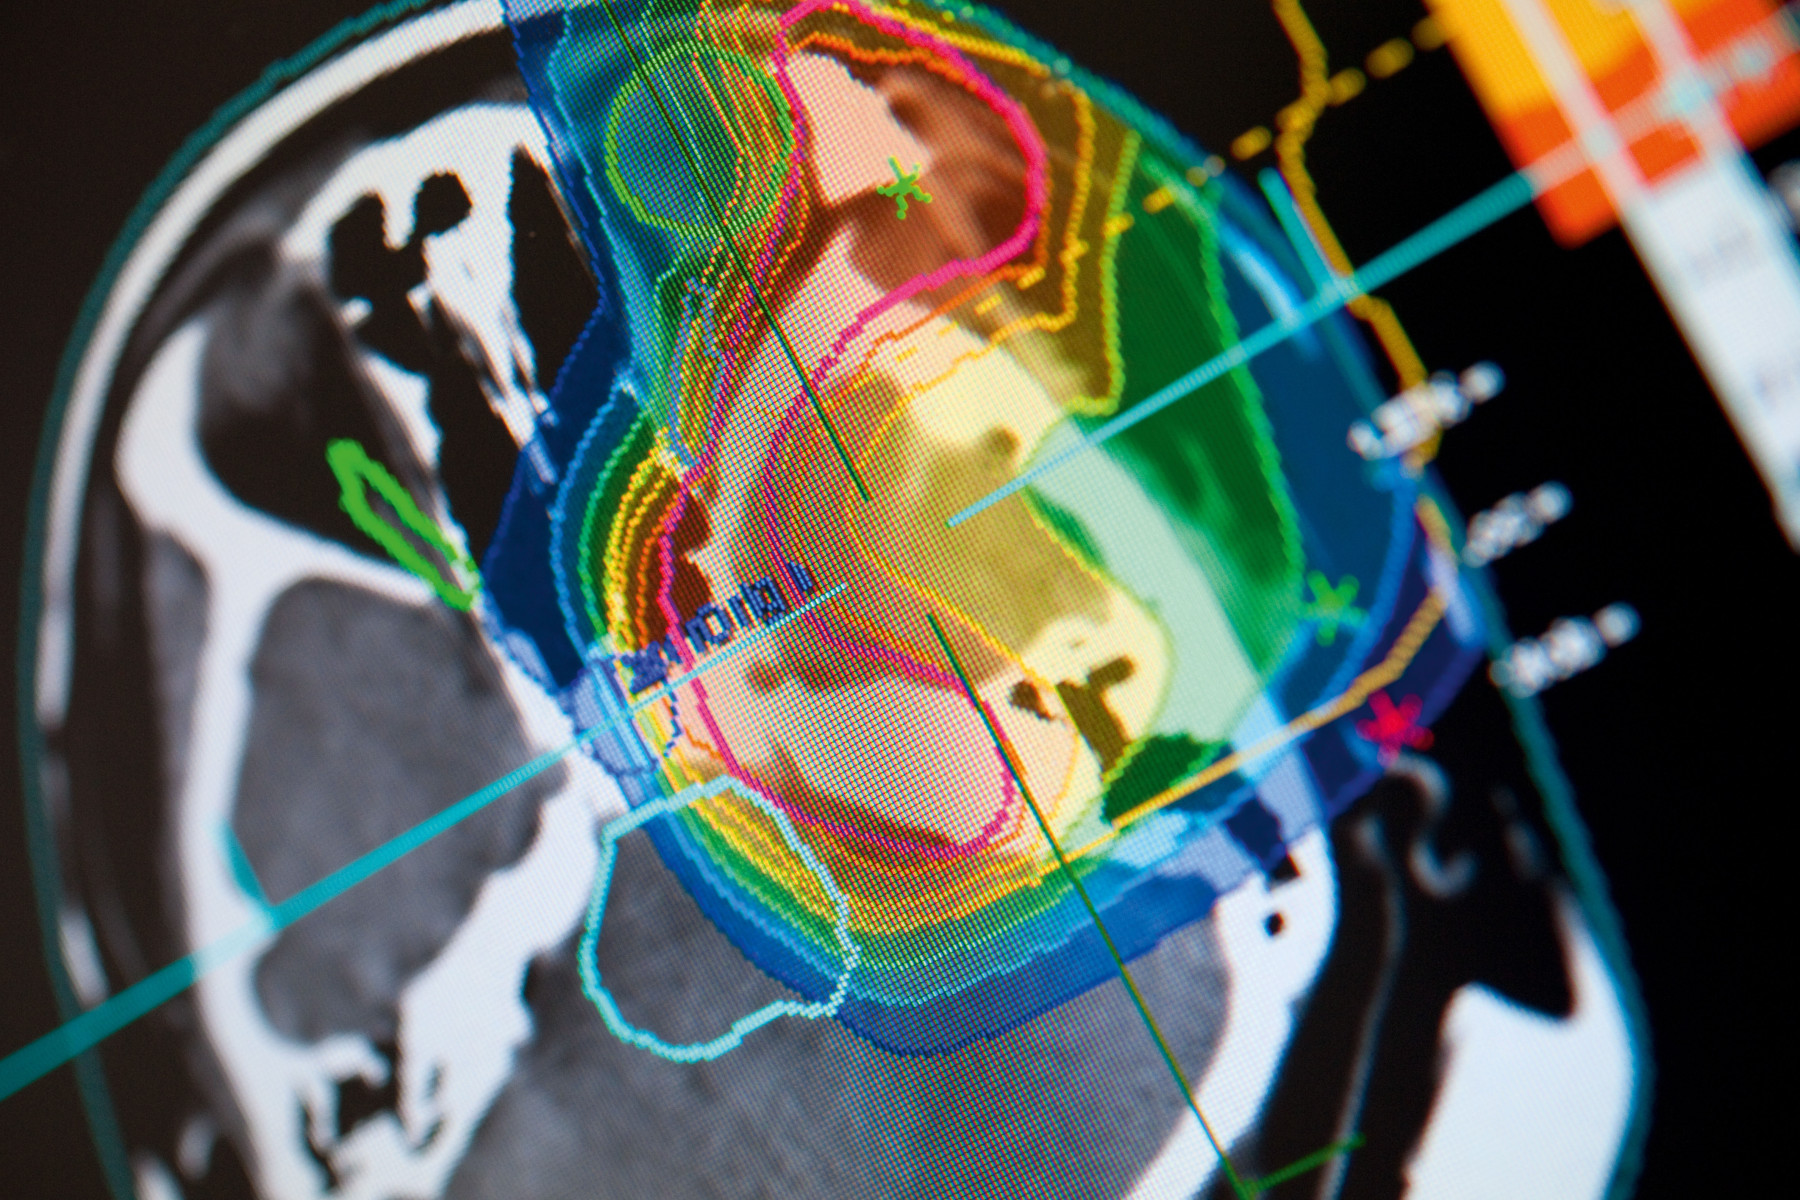
\includegraphics[width=0.9\textwidth]{Images/1920_hirntumorbestrahlung.jpg}
      \end{figure}
    \pause
  \begin{tikzpicture}[remember picture, overlay]
          \fill[black] (current page.south west) rectangle (current page.north east);
        \end{tikzpicture}
\end{frame}

 % Bibliography    
  \begin{frame}[allowframebreaks, noframenumbering, plain]{Literaturverzeichnis}
   \nocite{*}
   \printbibliography
  \end{frame}

\end{document}
